\documentclass{article}
\usepackage{graphicx} % Required for inserting images
\usepackage{subcaption} % Required for side-by-side subfigures
\graphicspath{ {./figures/} } % Tells LaTeX to look inside the figures folder
\usepackage{amsmath}
\usepackage{amssymb}


\title{CS 138 Assignment 1}
% {Multi-Armed Bandits in Non-Stationary Settings}
\author{Jiyeon Byun}
\date{October 6 2026}

\begin{document}

\maketitle

\begin{abstract}
    In non-stationary environment where actual values are not fixed, two
    different agents, the $\varepsilon$-greedy and the softmax, are implemented
    on multi-armed bandits. Other than the standard random-walk, two additional
    designs were implemented: a Flip bandit, where the values of two arms are
    swapped abruptly at fixed intervals, and a Sinusoidal bandit, where the
    values vary periodically. The softmax agent achieves slightly higher average
    reward than the $\varepsilon$-greedy agent. This suggests value-directed
    exploration performs better in tracking changing values than uniform random
    exploration.
\end{abstract}

\section{Introduction}
Reinforcement learning differs from the supervised and unsupervised learning
where there are input datasets and learn the patterns behind it for models to
generalize. Reinforcement learning has three properties of states, actions, and
rewards where the agent will experience through environment, make actions, and
gain rewards to learn to decide better actions. Multi-armed bandit problems are
the simplest form of reinforcement learning where there are no consequences from
actions or consideration of different states. There are K actions, and the
chosen action will give rewards R. The agent's goal is to maximize this reward
function so it can update its policy and make optimal decisions. The stationary
multi-armed bandit problems will eventually converge when the process is
repeated infinitely many times. Non-stationary multi-armed bandit problems, on
the other hand gives changing rewards. In this report, non-stationary
multi-armed bandits will be simulated using a random walk to show rewards over
time and the percentage of optimal actions selected. Then the softmax action
selection and $\varepsilon$-greedy action selection with decaying $\varepsilon$
and decaying temperature will be compared. Lastly, two additional types of
non-stationary will be presented. One is flip bandit where the rewards of random
two arms are switched to one another. Another design is a sinusoidal bandit
where the true value constantly shifts based on the time step.

\section{Methods}
\subsection{Environment Design}
\label{sec:environment-design}
The environment is built around a base class, \texttt{BanditEnvironment}, which
defines the state shared by every environment variant: the number of actions
$k$, the true action values $q_*(a)$ (hidden from the agent), the current time
step $t$, and the reward model, under which the reward for action $a$ is drawn
from a Gaussian distribution with mean $q_*(a)$ and a fixed standard deviation
$\sigma_r$.

The base class exposes three methods to the agent. \texttt{n\_actions()} returns
the number of available actions ($k=10$ in our experiments).
\texttt{step(action)} returns the reward sampled for the chosen action, together
with a boolean indicating whether that action was optimal at the current time
step. Internally, the optimal action is determined by $\arg\max_a q_*(a)$; this
value is used only to compute the boolean returned by \texttt{step()} and is
never exposed to the agent directly, preserving the information barrier between
environment and agent.

One hyperparameter of the base environment is the reward standard deviation
$\sigma_r$. Figure~\ref{fig:reward_variation} compares an $\varepsilon$-greedy
agent on the standard random-walk bandit under two settings: $\sigma_r = 0.1$
(left) and $\sigma_r = 1.0$ (right). A smaller $\sigma_r$ produces less noisy,
more visually interpretable reward curves. Therefore, $\sigma_r = 0.1$ is fixed
for all experiments reported here.

\begin{figure}[htbp]
    \centering
    \begin{subfigure}[t]{0.48\textwidth}
        \centering
        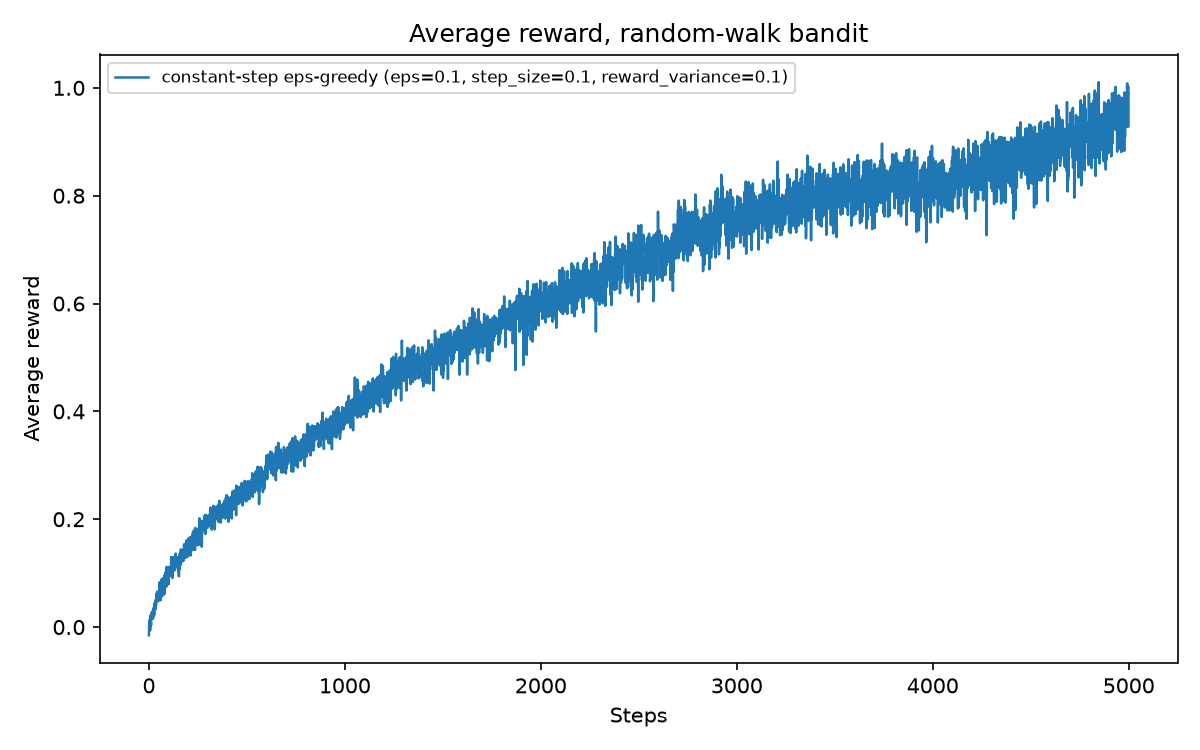
\includegraphics[width=\textwidth]{part0_reward_0.png}
        \caption{$\sigma_r = 0.1$}
    \end{subfigure}
    \hfill
    \begin{subfigure}[t]{0.48\textwidth}
        \centering
        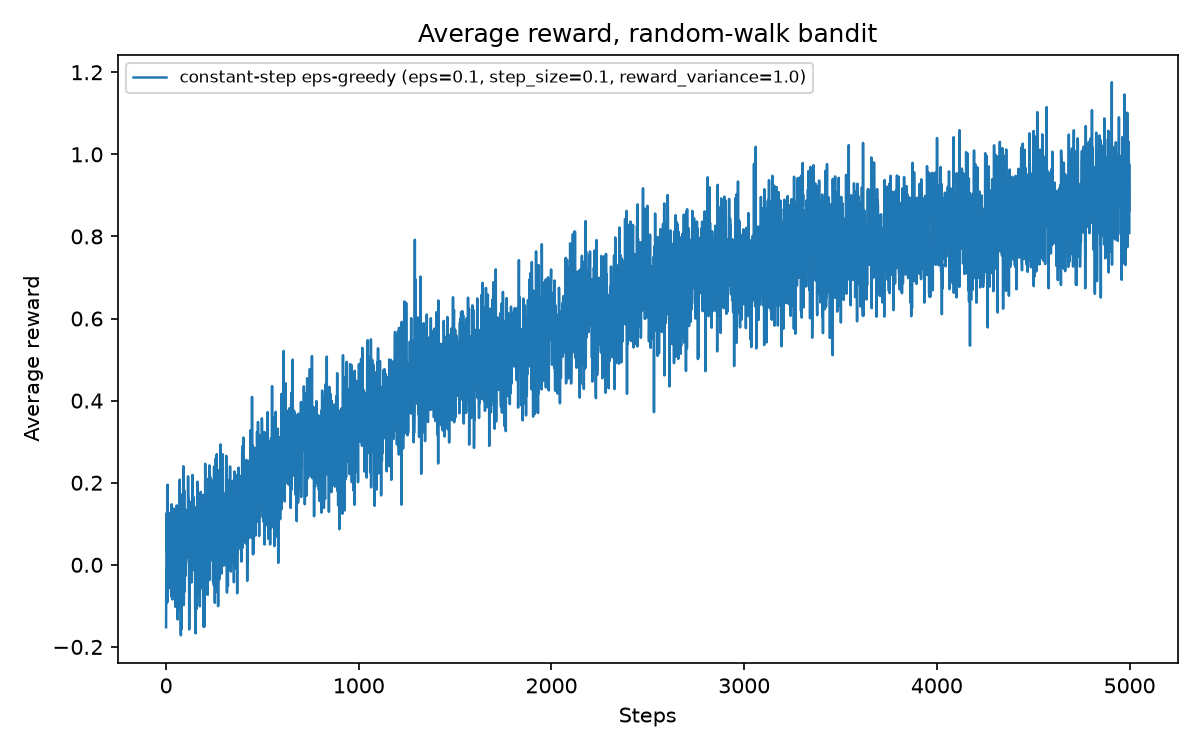
\includegraphics[width=\textwidth]{part0_reward_1.png}
        \caption{$\sigma_r = 1.0$}
    \end{subfigure}
    \caption{Effect of the reward standard deviation $\sigma_r$ on an
        $\varepsilon$-greedy agent in the standard random-walk bandit. A lower
        $\sigma_r$ (a) yields smoother curves than a higher $\sigma_r$ (b).
        $\sigma_r = 0.1$ is used throughout this report for visibility.}
    \label{fig:reward_variation}
\end{figure}

\subsection{Agent Design}
\label{sec:agent-design}
The base class, \texttt{Agent}, holds the variables shared by every agent
variant: the number of actions $k$, an initial value used to optimistically or
neutrally initialize $Q(a)$, a count $N(a)$ of how many times each action has
been chosen, the step size $\alpha$, and the current time step $t$. The base
class defines two methods that every subclass must implement or inherit:
\texttt{select\_action()}, which chooses an action given the agent's current
estimates, and \texttt{update(action, reward)}, which updates those estimates
after observing a reward. Keeping \texttt{select\_action()} abstract at the
base-class level lets different action-selection strategies share identical
update logic, so the two concerns do not become entangled in a single class.

The shared \texttt{update()} method increments $N(a)$ and $t$ by 1, then updates
the action-value estimate using a constant step size $\alpha$:
\begin{equation}
    Q_{n+1} = Q_n + \alpha \big( R_n - Q_n \big).
    \label{eq:constant_update}
\end{equation}
A constant $\alpha$ gives exponentially more weight to recent rewards than to
old ones, which is important in a non-stationary environment where old reward
information can become stale.

In Figure~\ref{fig:initial_value}, two initial values are compared for the
action-value estimates $Q(a)$ on an $\varepsilon$-greedy agent in the standard
random-walk bandit: $Q_0 = 0.0$ (left) and $Q_0 = 100$ (right). We use $Q_0 =
0.0$ throughout this report to isolate the effect of $\varepsilon$ from
optimistic-initialization exploration.

\begin{figure}[htbp]
    \centering
    \begin{subfigure}[t]{0.48\textwidth}
        \centering
        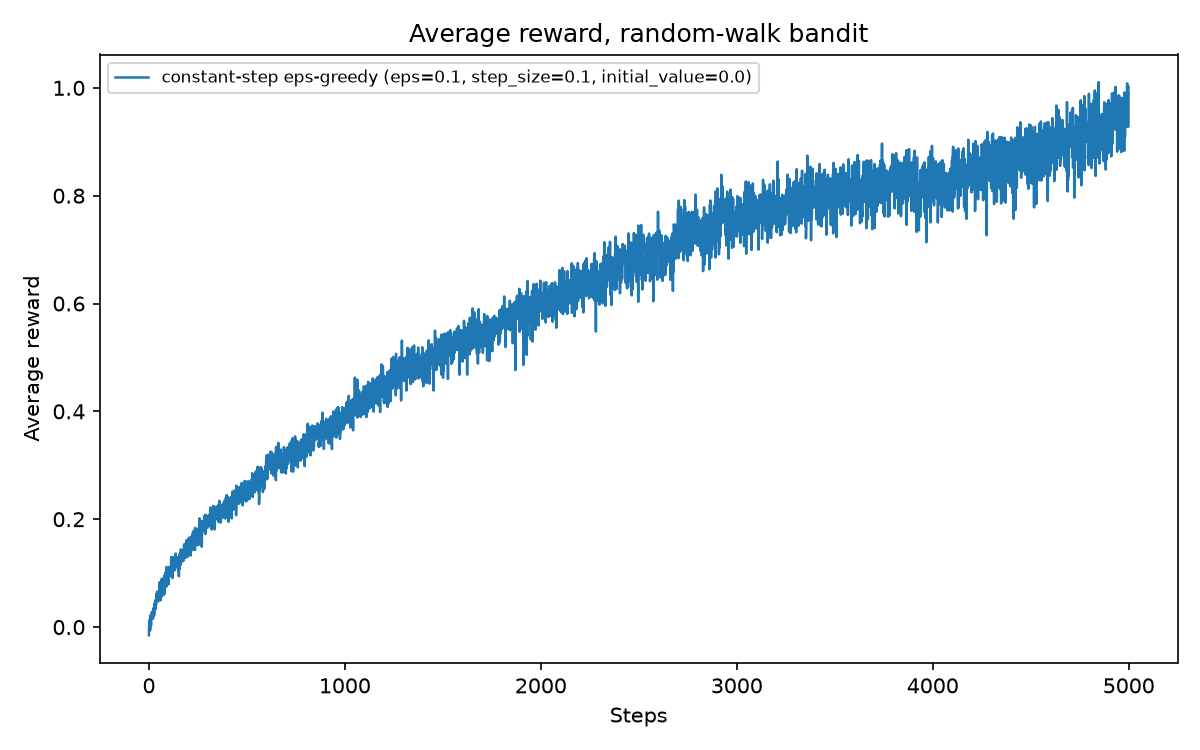
\includegraphics[width=\textwidth]{part0_reward_0_0.png}
        \caption{$Q_0 = 0.0$}
    \end{subfigure}
    \hfill
    \begin{subfigure}[t]{0.48\textwidth}
        \centering
        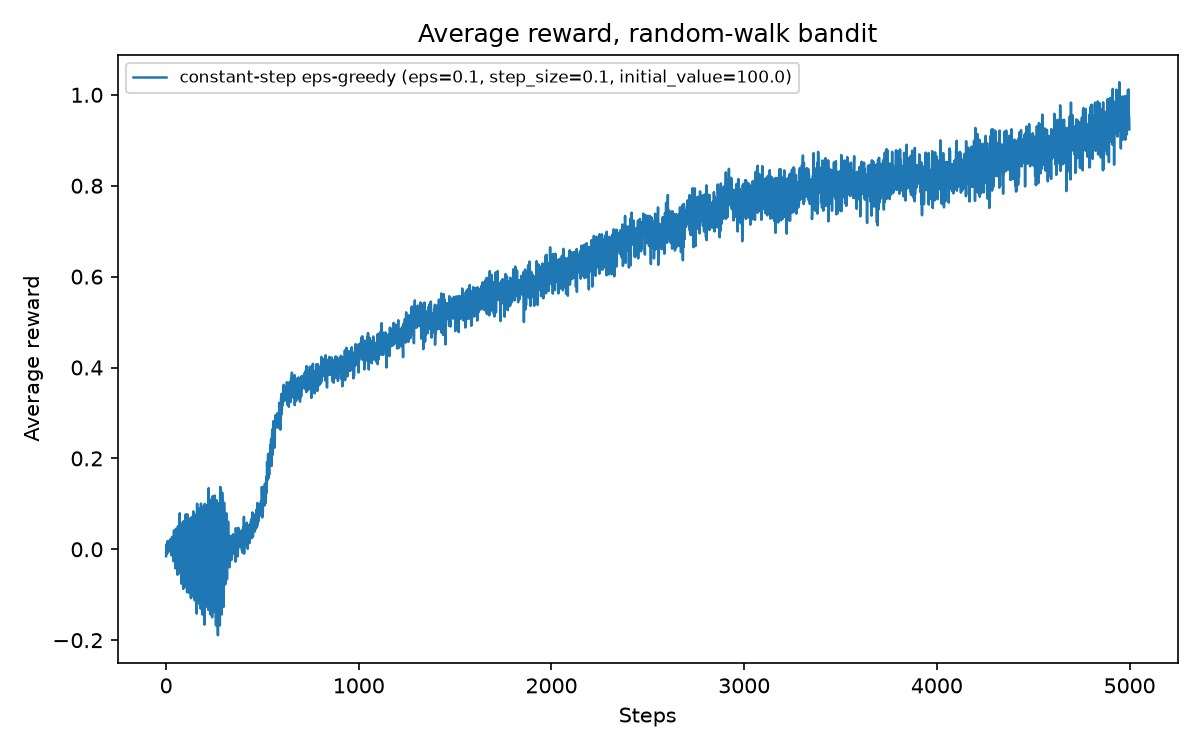
\includegraphics[width=\textwidth]{part0_reward_100.png}
        \caption{$Q_0 = 100$}
    \end{subfigure}
    \caption{Effect of the initial action-value estimate $Q_0$ on an
        $\varepsilon$-greedy agent in the standard random-walk bandit. The
        optimistic initialization $Q_0 = 100$ (b) forces early exploration
        compared to $Q_0 = 0.0$ (a). This is because agent gets disappointed as
        initial value is far higher than the true value and tries other
        actions.}
    \label{fig:initial_value}
\end{figure}

\subsection{Experimental Setup}
All experiments are run from a separate script that fixes $k=10$ arms, $T=5000$
time steps per run, and averages results over $N=150$ independent runs. Unless
otherwise noted, we use the default hyperparameters established in
Sections~\ref{sec:environment-design} and~\ref{sec:agent-design}: reward
standard deviation $\sigma_r = 0.1$, initial action-value estimate $Q_0 = 0.0$,
and step size $\alpha = 0.1$.

The experiment script defines three functions that implement this procedure.
\texttt{run\_single()} runs one agent on one environment instance for $T$ steps.
At each step, it calls the environment's \texttt{step()} function to obtain a
reward and whether the chosen action was optimal, passes the reward to the
agent's \texttt{update()} function to update its $Q$ estimates, and records both
values. It returns the full reward and optimality sequences for that run.
\texttt{average\_over\_runs()} calls \texttt{run\_single()} $N$ times, each with
a different random seed, and returns the mean reward and mean percentage of
optimal actions at each time step across runs. \texttt{plot\_curves} is a
plotting helper that takes one or more of these averaged curves and renders them
on a shared set of axes for comparison.

Averaging over $N=150$ runs reduces the variance introduced by the stochastic
reward signal and by each agent's own exploration, so that the resulting curves
reflect the behavior of a method rather than the noise of a single run.

\section{Non-stationary MABs via Random Walk}
\label{sec:part1}

\subsection{Random Walk and Epsilon-Greedy Action Selection}
The random-walk environment is implemented with all $q_*(a)$ initialized to 0,
after which each $q_*(a)$ independently takes a normal random walk step with
standard deviation $\sigma_{\text{walk}} = 0.01$ at every time step.
\texttt{EpsilonGreedyAgent} selects the greedy action $\arg\max_a Q(a)$ with
probability $1-\varepsilon$, and a random action with probability $\varepsilon$.
Ties among greedy actions are broken at random, rather than always selecting the
lowest-indexed action, to avoid a systematic selection bias early in training
when many $Q$ values are equal. For this section, we use a \emph{fixed}
$\varepsilon = 0.1$.

\subsection{Constant step-size method vs. sample-average method}
Two different update rules are compared for the $\varepsilon$-greedy agent. The
first is the constant step-size update of Eq.~\eqref{eq:constant_update} with
$\alpha = 0.1$. The second is the sample-average update,

\begin{equation}
    Q_{n+1} = Q_{n} + \frac{1}{n} \Big[ R_n - Q_n \Big],
    \label{eq:sample_average_update}
\end{equation}

\noindent where $n$ is the number of times an action has been selected.

\begin{figure}[h!]
    \centering
    \begin{subfigure}{0.48\textwidth}
        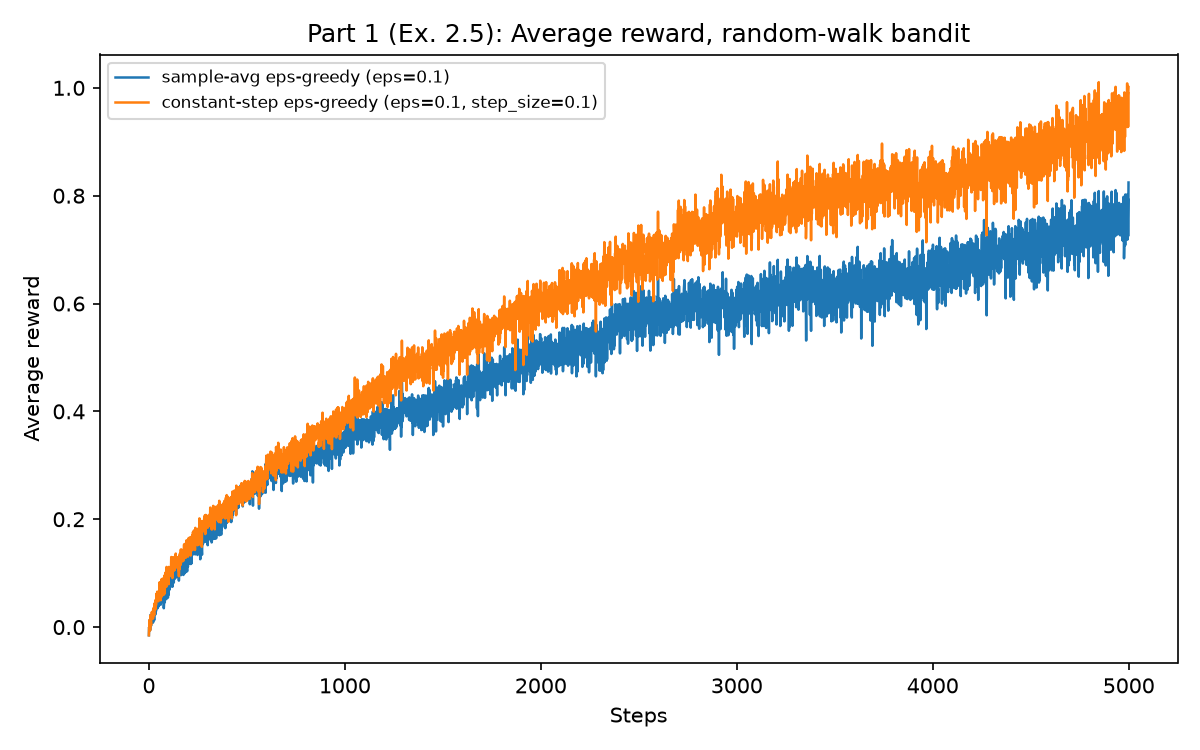
\includegraphics[width=\textwidth]{part1_reward.png}
        \caption{Average reward over time.}
    \end{subfigure}
    \hfill
    \begin{subfigure}{0.48\textwidth}
        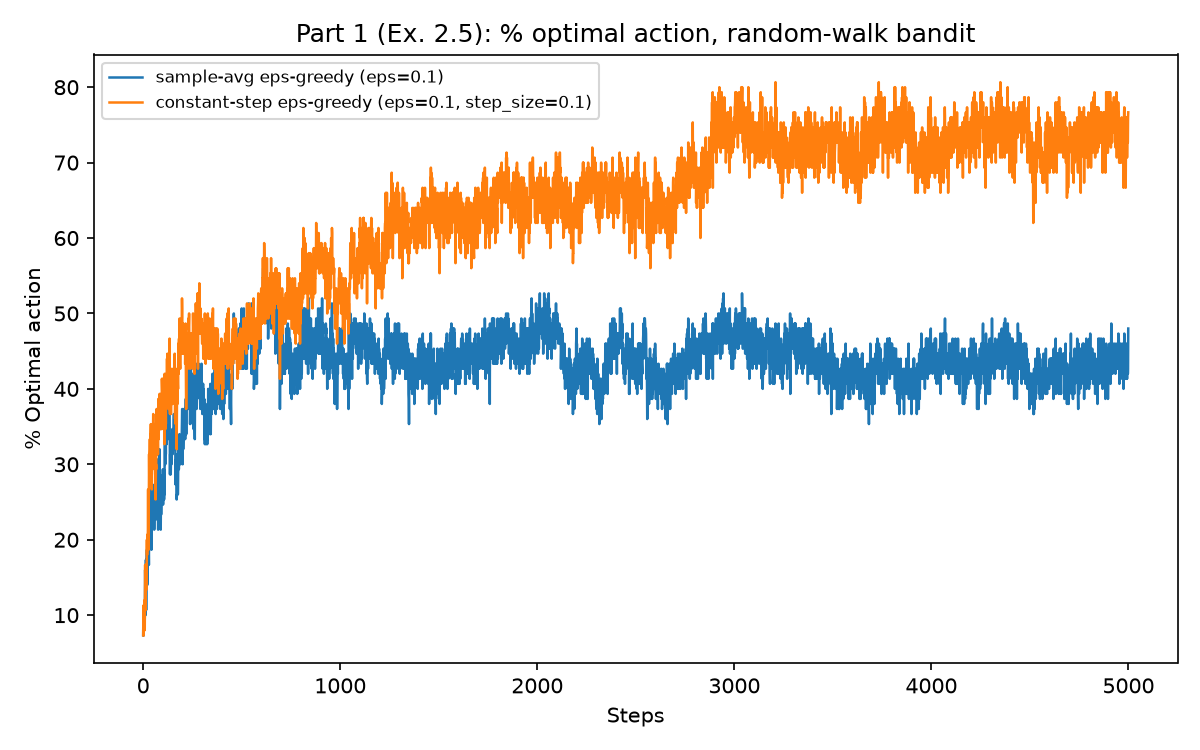
\includegraphics[width=\textwidth]{part1_optimal.png}
        \caption{\% optimal action selected over time.}
    \end{subfigure}
    \caption{Results on the random-walk bandit, simulated for 5000 steps
        averaged over 150 runs. (a) Average reward over time. (b) \% optimal
        action selected over time. The orange line uses the constant-step update
        (Eq.~\eqref{eq:constant_update}); the blue line uses the sample-average
        update (Eq.~\eqref{eq:sample_average_update}).}
    \label{fig:part1}
\end{figure}

As Figure~\ref{fig:part1}(a) shows, the sample-average method performs worse on
this non-stationary problem than the constant-step method. This follows directly
from the two update rules. In Eq.~\eqref{eq:sample_average_update}, the
effective step size is $1/n$, which shrinks toward zero as an action is selected
more often. After many selections, a new reward impacts $Q(a)$ less, making it
converge to an average over the action's \emph{entire} selection history.
However, because $q_*(a)$ is drifting via the random walk, old rewards does not
reflect the current rewards accurately. So an averaged estimate becomes a poor
estimate of the action's \emph{current} value. In
Eq.~\eqref{eq:constant_update}, by contrast, the step size $\alpha$ is fixed and
does not shrink with $n$, which gives every update exponentially more weight to
recent rewards over old ones. This lets $Q(a)$ continue tracking $q_*(a)$ as it
drifts, rather than converging to a fixed point. This can be shown in the
equation:
\begin{equation}
    Q_{n+1} = (1-\alpha)^nQ_{1} + \sum_{i=1}^{n} \alpha(1-\alpha)^{n-i}R_i,
    \label{eq:constant_update_expanded}
\end{equation}

This same mechanism explains why percentage optimal action
Figure~\ref{fig:part1}(b) degrades for the sample-average agent. Because the
sample-average agent's $Q$ estimates lag behind the true, drifting $q_*(a)$, the
action with the highest \emph{estimated} value gradually differs from the action
with the highest \emph{true} value. Therefore, both average reward and
percentage optimal action show that stale value estimates cause the agent to
select non-optimal actions.

\section{Softmax Exploration}
\label{sec:part2}

\subsection{Softmax Action Selection}
\texttt{SoftmaxAgent} selects actions stochastically in proportion to the
estimated value of $Q$:
\begin{equation}
    P(a) = \frac{\exp\!\big(Q(a)/\tau\big)}{\sum_{b} \exp\!\big(Q(b)/\tau\big)},
    \label{eq:softmax}
\end{equation}
where the temperature $\tau$ controls the randomness to balance exploitation and
exploration. As $\tau \to 0$, the probability assigned to the highest-valued
action approaches 1, resulting in exploitation. As $\tau \to \infty$, all
actions approach equal probability of being chosen, resulting in exploration.

\subsection{Decaying $\varepsilon$ and $\tau$}
This section compares two agent variants on the random-walk bandit of
Section~\ref{sec:part1}: $\varepsilon$-greedy with decaying $\varepsilon$, and
softmax with decaying $\tau$. Both use the same hyperbolic decay schedule,
\begin{equation}
    x_t = \max\!\left(x_{\min},\
    \frac{x_0}{1 + \beta t}\right),
    \label{eq:decay-schedule}
\end{equation}
applied with $x = \varepsilon$ for $\varepsilon$-greedy and $x = \tau$ for
softmax. Here $x_0$ is the initial rate, $\beta$ controls how quickly the rate
decays, and $x_{\min}$ is a floor that preserves a small amount of exploration
indefinitely. Both schedules are initialized with $x_0 = 1.0$, $\beta = 0.005$,
and $x_{\min} = 0.01$, chosen so that exploration falls off gradually over the
course of a run while still preserving enough residual exploration for the agent
to keep adapting to the non-stationary environment.

\begin{figure}[h!]
    \centering
    \begin{subfigure}{0.48\textwidth}
        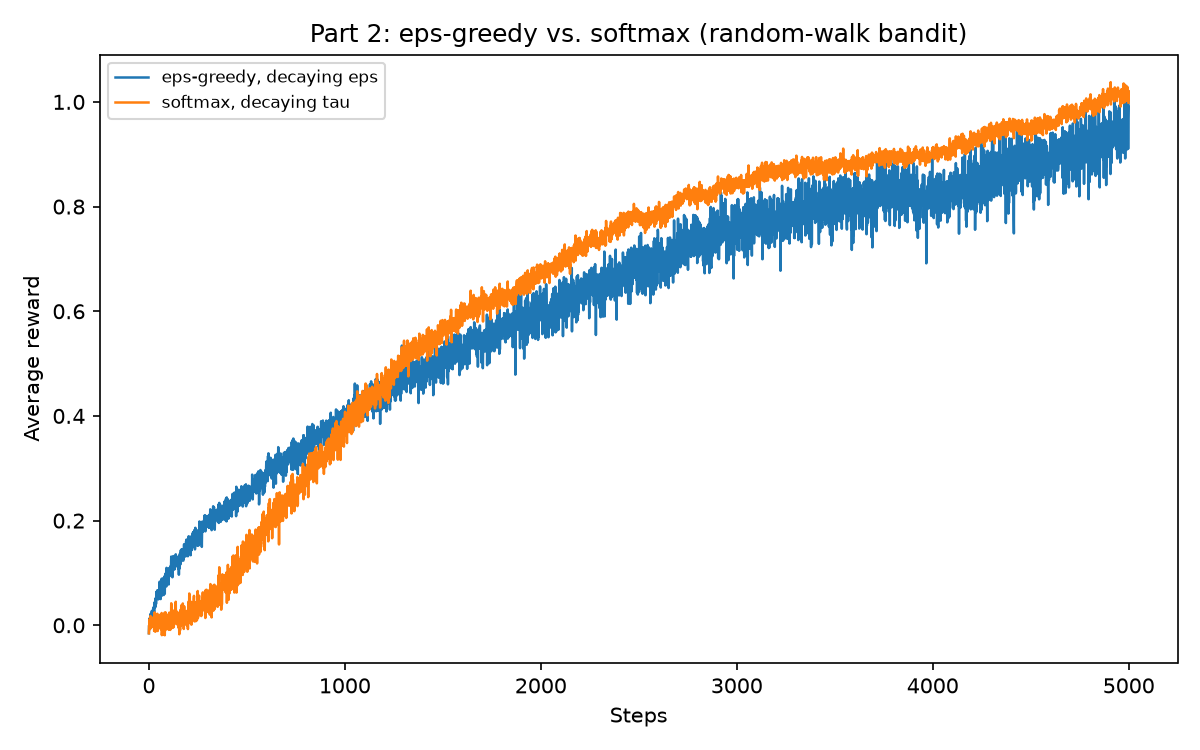
\includegraphics[width=\textwidth]{figures/part2_reward.png}
        \caption{Average reward over time.}
    \end{subfigure}
    \hfill
    \begin{subfigure}{0.48\textwidth}
        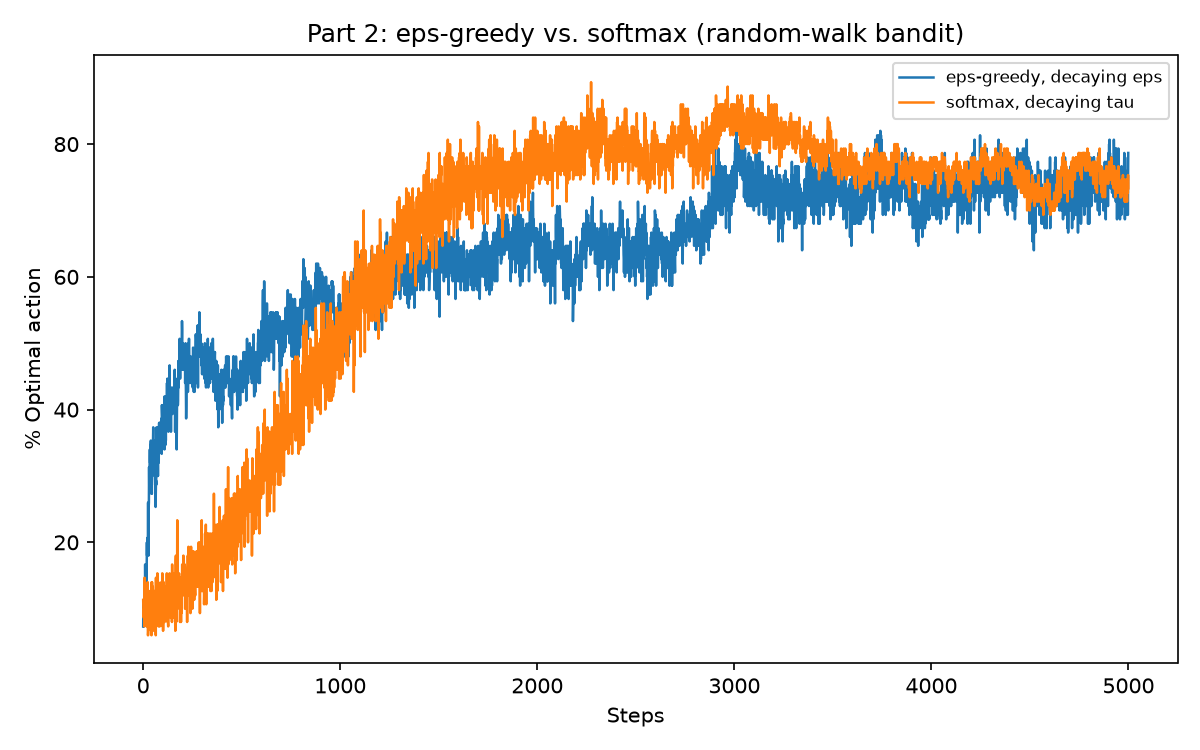
\includegraphics[width=\textwidth]{figures/part2_optimal.png}
        \caption{\% optimal action selected over time.}
    \end{subfigure}
    \caption{$\varepsilon$-greedy with decay $\varepsilon$ vs.\ softmax with
        decay on the random-walk bandit of Section~\ref{sec:part1}, simulated
        for 5000 steps averaged over 150 runs.}
    \label{fig:part2}
\end{figure}

\subsection{Discussion}
According to Figure~\ref{fig:part2}, the $\varepsilon$-greedy agent learns fast
in the early stage of training, whereas the softmax agent learns slowly at first
but later crosses over the $\varepsilon$-greedy agent. This is unlikely due to
the rate of decay as both decay calculation uses same equation, Eq
\ref{eq:decay-schedule}. A more plausible explanation lies in the systematic
design of $\varepsilon$-greedy agent and the softmax agent. When
$\varepsilon$-greedy agent decides to be greedy, it deterministically chooses
the current optimal action. On the other hand, the softmax samples the actions
with probabilities based on the estimated values, which causes the softmax agent
to choose less optimal actions. During the early phase of the training, the
initial estimates of actions are identical. So the softmax agent spends more
time with low-value actions, making it look slow in learning in comparison to
the $\varepsilon$-greedy agent. However, this early exploration helps the
softmax function in later phase of the training, as it will gradually focus more
on higher estimates. Therefore, the softmax agent can gradually catch up and
perform even better as the training continues.

\section{Other Types of Non-stationarity}
\label{sec:part3}
In section \ref{sec:part1}, non-stationarity was established by drifting $q_*$
function with a small deviation. In this section, two additional types of
non-stationary settings are introduced: flip bandit and sinusoidal bandit. To
reduce the noise of the plots, this section uses $\varepsilon, \tau = 0.1$
unlike 1.0 from Section~\ref{sec:part2}

\subsection{Flip Bandit}
This environment starts with a standard 10-armed testbed. The sudden change
comes in every 1000 steps to switch the true action values of two randomly
picked arms. Compared to the initial set up of non-stationarity shown in section
\ref{sec:part1}, flip implementation is more abrupt and and discrete. In this
environment, both $\varepsilon$-greedy agent and softmax agents are implemented,
but the agents will not experience any decay and the $\varepsilon$ and $\tau$
are set to 0.1.

\begin{figure}[h!]
    \centering
    \begin{subfigure}{0.48\textwidth}
        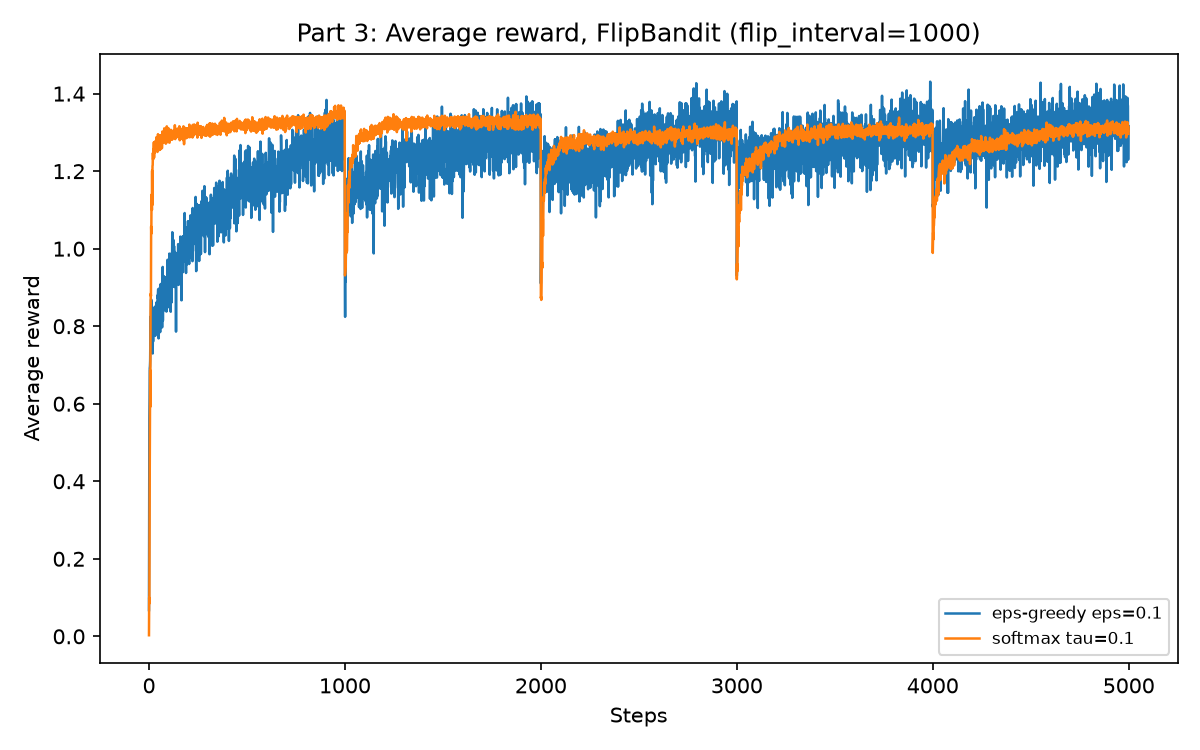
\includegraphics[width=\textwidth]{figures/part3_FlipBandit_reward.png}
        \caption{Average reward.}
    \end{subfigure}
    \hfill
    \begin{subfigure}{0.48\textwidth}
        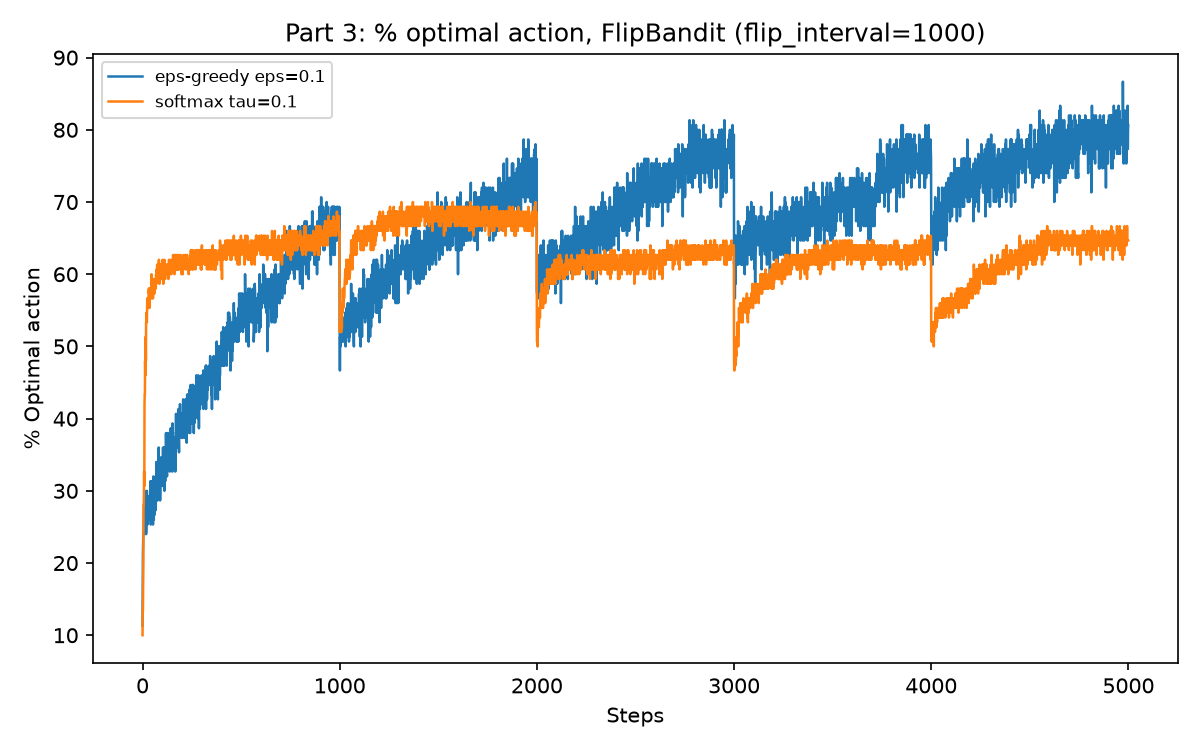
\includegraphics[width=\textwidth]{figures/part3_FlipBandit_optimal.png}
        \caption{\% optimal action.}
    \end{subfigure}
    \caption{$\varepsilon$-greedy agent and softmax agents with constant
        hyperparameter on flip non-stationary environment. After each flip,
        softmax learns faster at the start, whereas $\varepsilon$-greedy yields
        higher optimal-action rate.}
    \label{fig:part3-flip}
\end{figure}

As shown in Figure~\ref{fig:part3-flip}, both $\varepsilon$-greedy agent and
softmax agent experience a sudden drop every 1000 steps. After the flip, both
agents selects outdated actions receiving non-optimal rewards, which causes the
drop. This drop is only temporary as both agents continue to explore and recover
by learning to estimate updated values again.

In this fixed $\varepsilon$ and $\tau$ settings, the softmax agent learns much
faster in the beginning of the simulation. After each flip, softmax agent tends
to recover much faster than $\varepsilon$-greedy agent. However,
$\varepsilon$-greedy reaches higher percentage optimal action compared to the
softmax function. A likely explanation would be that softmax concentrates on
near-optimal arms, which yield high reward without being the best arm, whereas
$\varepsilon$-greedy selects the best arm more often but also wastes exploratory
steps uniformly on poor arms. Because softmax rarely samples arms it currently
rates as poor, it may also be slower to discover that an arm has become optimal
after a flip, which is consistent with its lower percentage optimal.

\subsection{Sinusoidal Bandit}
Sinusoidal bandit also starts with 10-arm bandit testbed setup. In contrast to
the flip, this implementation will experience continuous change in rewards based
one steps. First, \textit{period} T is set to be 1000 so that one sine wave
completes every 1000 steps, and \textit{phase} are randomly assigned to the 10
arms ranging from 0 to $2\pi$. Then, $q_*(a)$ is defined as:
\begin{equation}
    q^*_k(t) = \sin\left(\frac{2\pi t}{T} + \phi_k\right),\qquad \phi_k \sim \mathcal{U}(0, 2\pi), \quad k = 1, \dots, K
    \label{eq:sinusoidal}
\end{equation}
where t represents the steps. Once assigned, it will automatically shift the
true values based on the current time steps. Similar to the flip bandit, both
$\varepsilon$-greedy and softmax agents are implemented without the decay.

\begin{figure}[h!]
    \centering
    \begin{subfigure}{0.48\textwidth}
        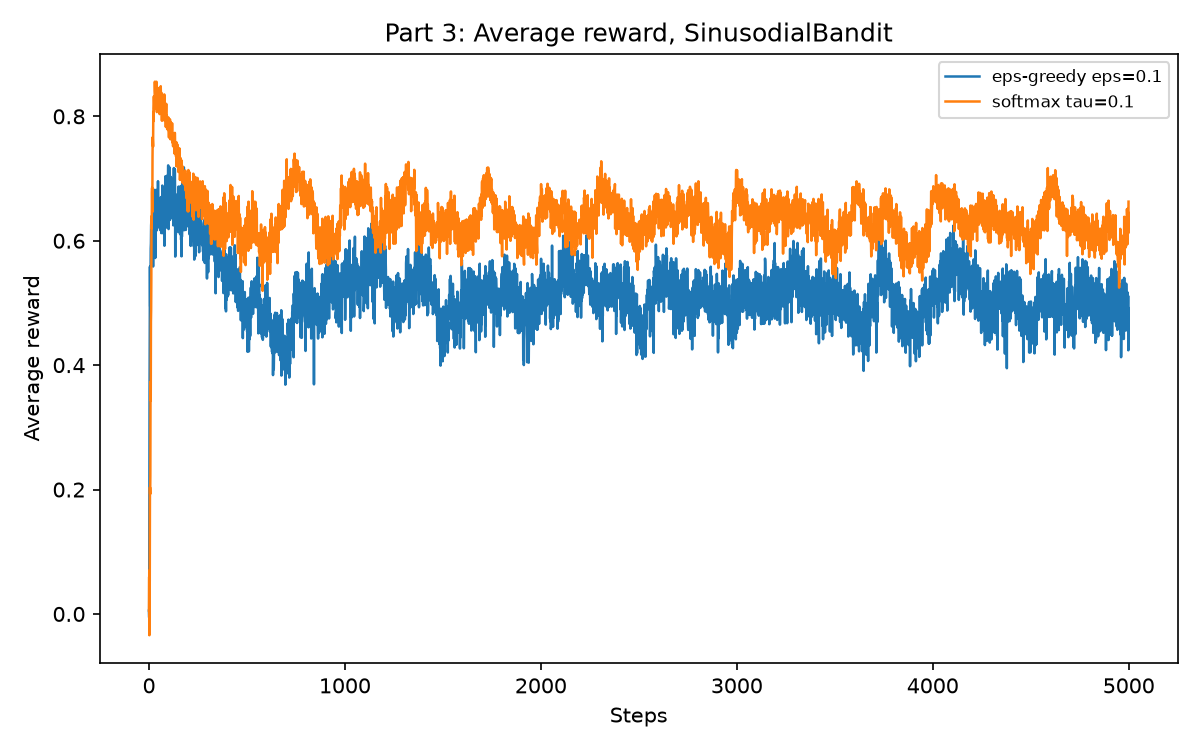
\includegraphics[width=\textwidth]{figures/part3_SinusodialBandit_reward.png}
        \caption{Average reward.}
    \end{subfigure}
    \hfill
    \begin{subfigure}{0.48\textwidth}
        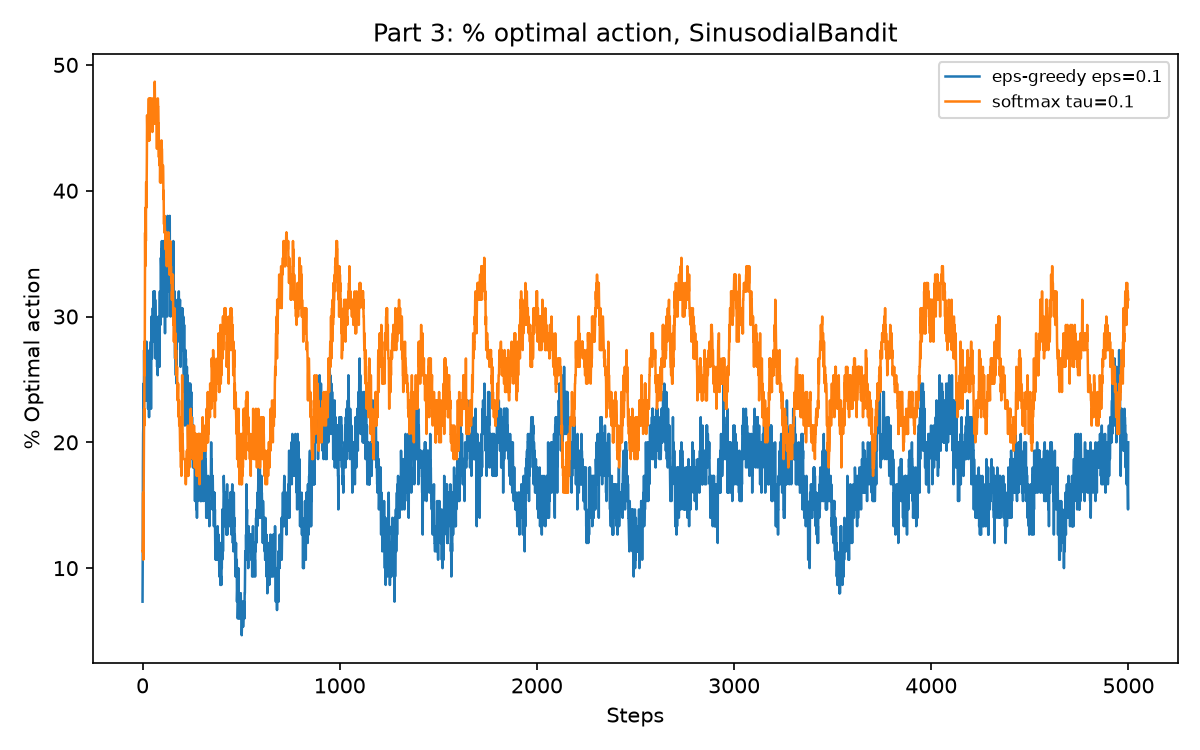
\includegraphics[width=\textwidth]{figures/part3_SinusodialBandit_optimal.png}
        \caption{\% optimal action.}
    \end{subfigure}
    \caption{$\varepsilon$-greedy agent and softmax agents with constant
        hyperparameter on sinusoidal non-stationary environment. Both agents
        continuously fluctuates. Softmax learns performs better than
        $\varepsilon$-greedy agent by exploring near optimal choices.}
    \label{fig:part3-sinusoidal}
\end{figure}

Compared to the flip bandit, there are no sudden and abrupt drop on the
Figure~\ref{fig:part3-sinusoidal}. Instead, the graphs are continuously
fluctuating because the true value constantly shifts based on the steps. In the
sinusoidal bandit, the softmax agent outperforms the $\varepsilon$-greedy agent.
This is likely due to the greedy actions are constantly outdated, whereas
softmax agent's sampling helps it to explore the choices close to optimal
action.

\subsection{Hyperparameter comparison}
In this section, the impact of step size is examined and showcased in the flip
environment using $\varepsilon$-greedy agent with decaying rate of 0.005. The
chosen hyperparameter values are 0.02, 0.1, 0.3, and 0.5.

\begin{figure}[h!]
    \centering
    \begin{subfigure}{0.48\textwidth}
        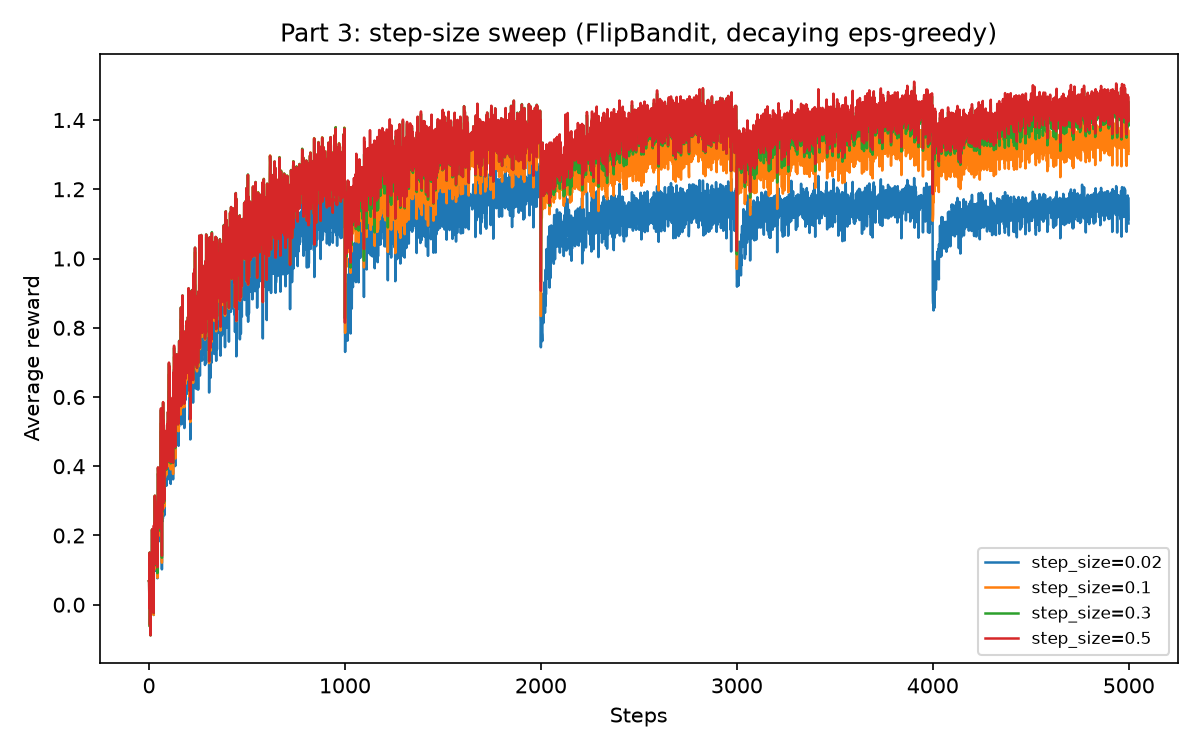
\includegraphics[width=\textwidth]{figures/part3_alpha_sweep_reward.png}
        \caption{Average reward.}
    \end{subfigure}
    \hfill
    \begin{subfigure}{0.48\textwidth}
        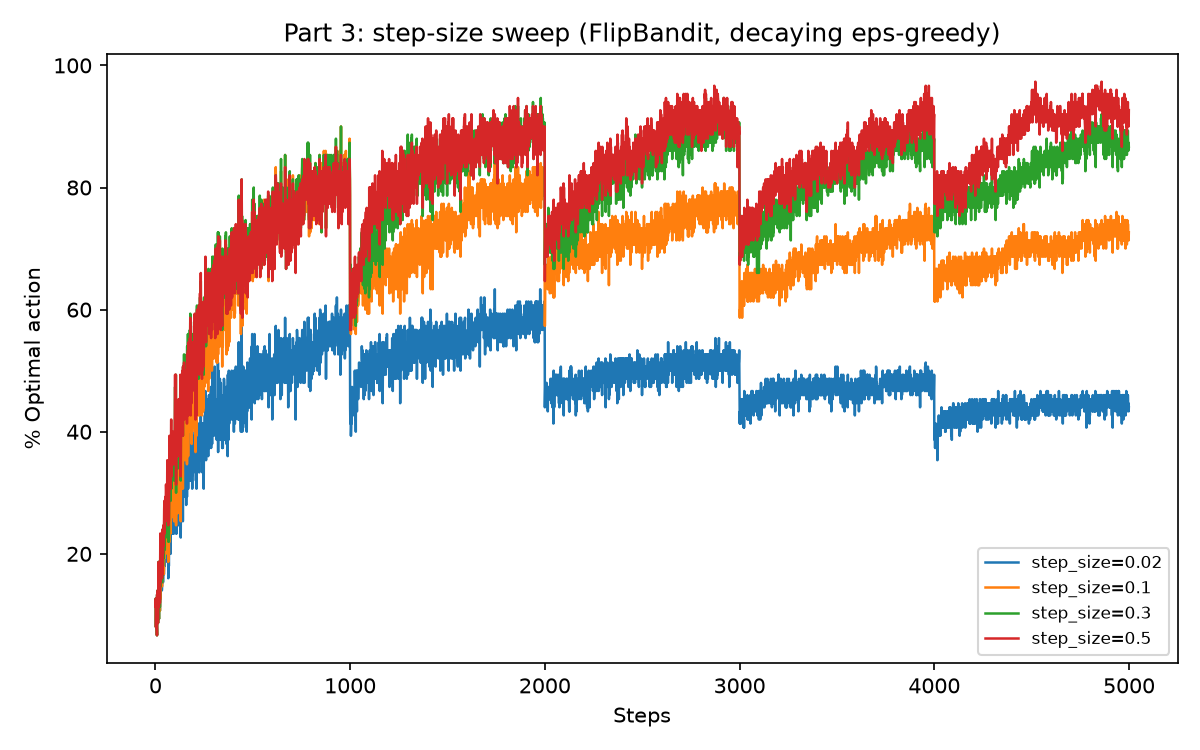
\includegraphics[width=\textwidth]{figures/part3_alpha_sweep_optimal.png}
        \caption{\% optimal action.}
    \end{subfigure}
    \caption{Effect of step size $\alpha$ under The flip bandit environment. The
        higher step size makes the agent more resilient to sudden change in the
        sense that it could update the policy to choose high percentage optimal
        action.}
    \label{fig:part3-alpha}
\end{figure}

The step-size sweep reveals a classic adaptivity on the FlipBandit task. Large
constant step sizes ($\alpha$ = 0.3, 0.5) could track the sudden change after
the flip and recover the percentage optimal action quickly. The smaller step
sizes ($\alpha$ = 0.02, 0.1) perform worse than the bigger step sizes as they
weight past rewards more heavily. These past rewards, however, became obsolete
after the flip. Since the large step size weights past rewards less, they are
faster to recover.

\section{Conclusion}
In this report, different types of agents and environments were explored. The
$\varepsilon$-greedy agent learns faster in the beginning of the simulation, but
softmax agent performs better in the later phase as it focuses on high-value
estimates. With decaying epsilon, both agents slightly fall below as they
explore less. In terms of non-stationary environment, a standard random walk
environment was implemented to the flip environment with sudden true values swap
of two arms and to the sinusoidal environment where true values constantly
change in terms of the steps. Different values of step sizes were experimented
and larger step sizes recovered fastest after flips.

\section{Extra Credit}
\subsection*{Exercise 2.3}
The $\varepsilon = 0.01$ method performs best in the long run on both measures.
Once its estimates have converged, its greedy action is the optimal action:
\[
    P(\text{optimal}) = (1 - \varepsilon) + \frac{\varepsilon}{k},
\]
which for $k=10$ gives $0.991$ for $\varepsilon = 0.01$ versus $0.910$ for
$\varepsilon = 0.1$. The best arm earns $q_*(a^*) \approx 1.54$ on average and a
uniformly random arm earns $0$ in expectation. Then, the asymptotic expected
reward per step is $\mathbb{E}[R_t] = (1-\varepsilon)\cdot 1.54 + \varepsilon
\cdot 0$, which is about $1.52$ for $\varepsilon=0.01$ and $1.39$ for
$\varepsilon=0.1$. For cumulative rewards, the gap of roughly $0.14$ per step
grows linearly, to about $140$ extra reward units per $1000$ steps. The
$\varepsilon = 0.01$ curve is still rising at step $1000$ in Figure~2.2, so its
advantage only becomes visible beyond the plotted window.

\subsection*{Exercise 2.4}
With non-constant step sizes, the update is
\[
    Q_{n+1} = Q_n + \alpha_n (R_n - Q_n)
    = \alpha_n R_n + (1 - \alpha_n) Q_n.
\]
Expanding this equation to utilize the initial estimate $Q_1$ gives
\[
    Q_{n+1} = \Big(\prod_{j=1}^{n} (1-\alpha_j)\Big) Q_1 + \sum_{i=1}^{n} \alpha_i \Big(\prod_{j=i+1}^{n} (1-\alpha_j)\Big) R_i.
\]
Hence the weight on the prior reward $R_i$ is
\[
    w_i = \alpha_i \prod_{j=i+1}^{n}(1 - \alpha_j),
\]
the step size at the time the reward arrived, discounted by $(1 - \alpha_j)$ for
every later update $j$. The weight on $Q_1$ is $\prod_{j=1}^{n}(1-\alpha_j)$,
and all weights sum to $1$. So $Q_{n+1}$ remains a weighted average of $Q_1$ and
the past rewards. For a constant $\alpha_n = \alpha$ this reduces to the weights
$\alpha(1-\alpha)^{n-i}$ of (2.6), and for $\alpha_n = 1/n$ the product
telescopes to $w_i = 1/n$ for every $i$ while the weight on $Q_1$ vanishes
(since $\alpha_1 = 1$), recovering the sample average.
% =====================================================================
% Only include if you collaborated with classmates, per the syllabus's
% collaboration policy.
% =====================================================================
\section*{Collaboration}
I used ChatGPT in terms of writing the code, checking the math formula, and
formatting the LaTeX. All conversations are documented in ChatGPT\_log

\end{document}
